\chapter{Methodology} \label{chap:metodologia}

\begin{figure}
\centering
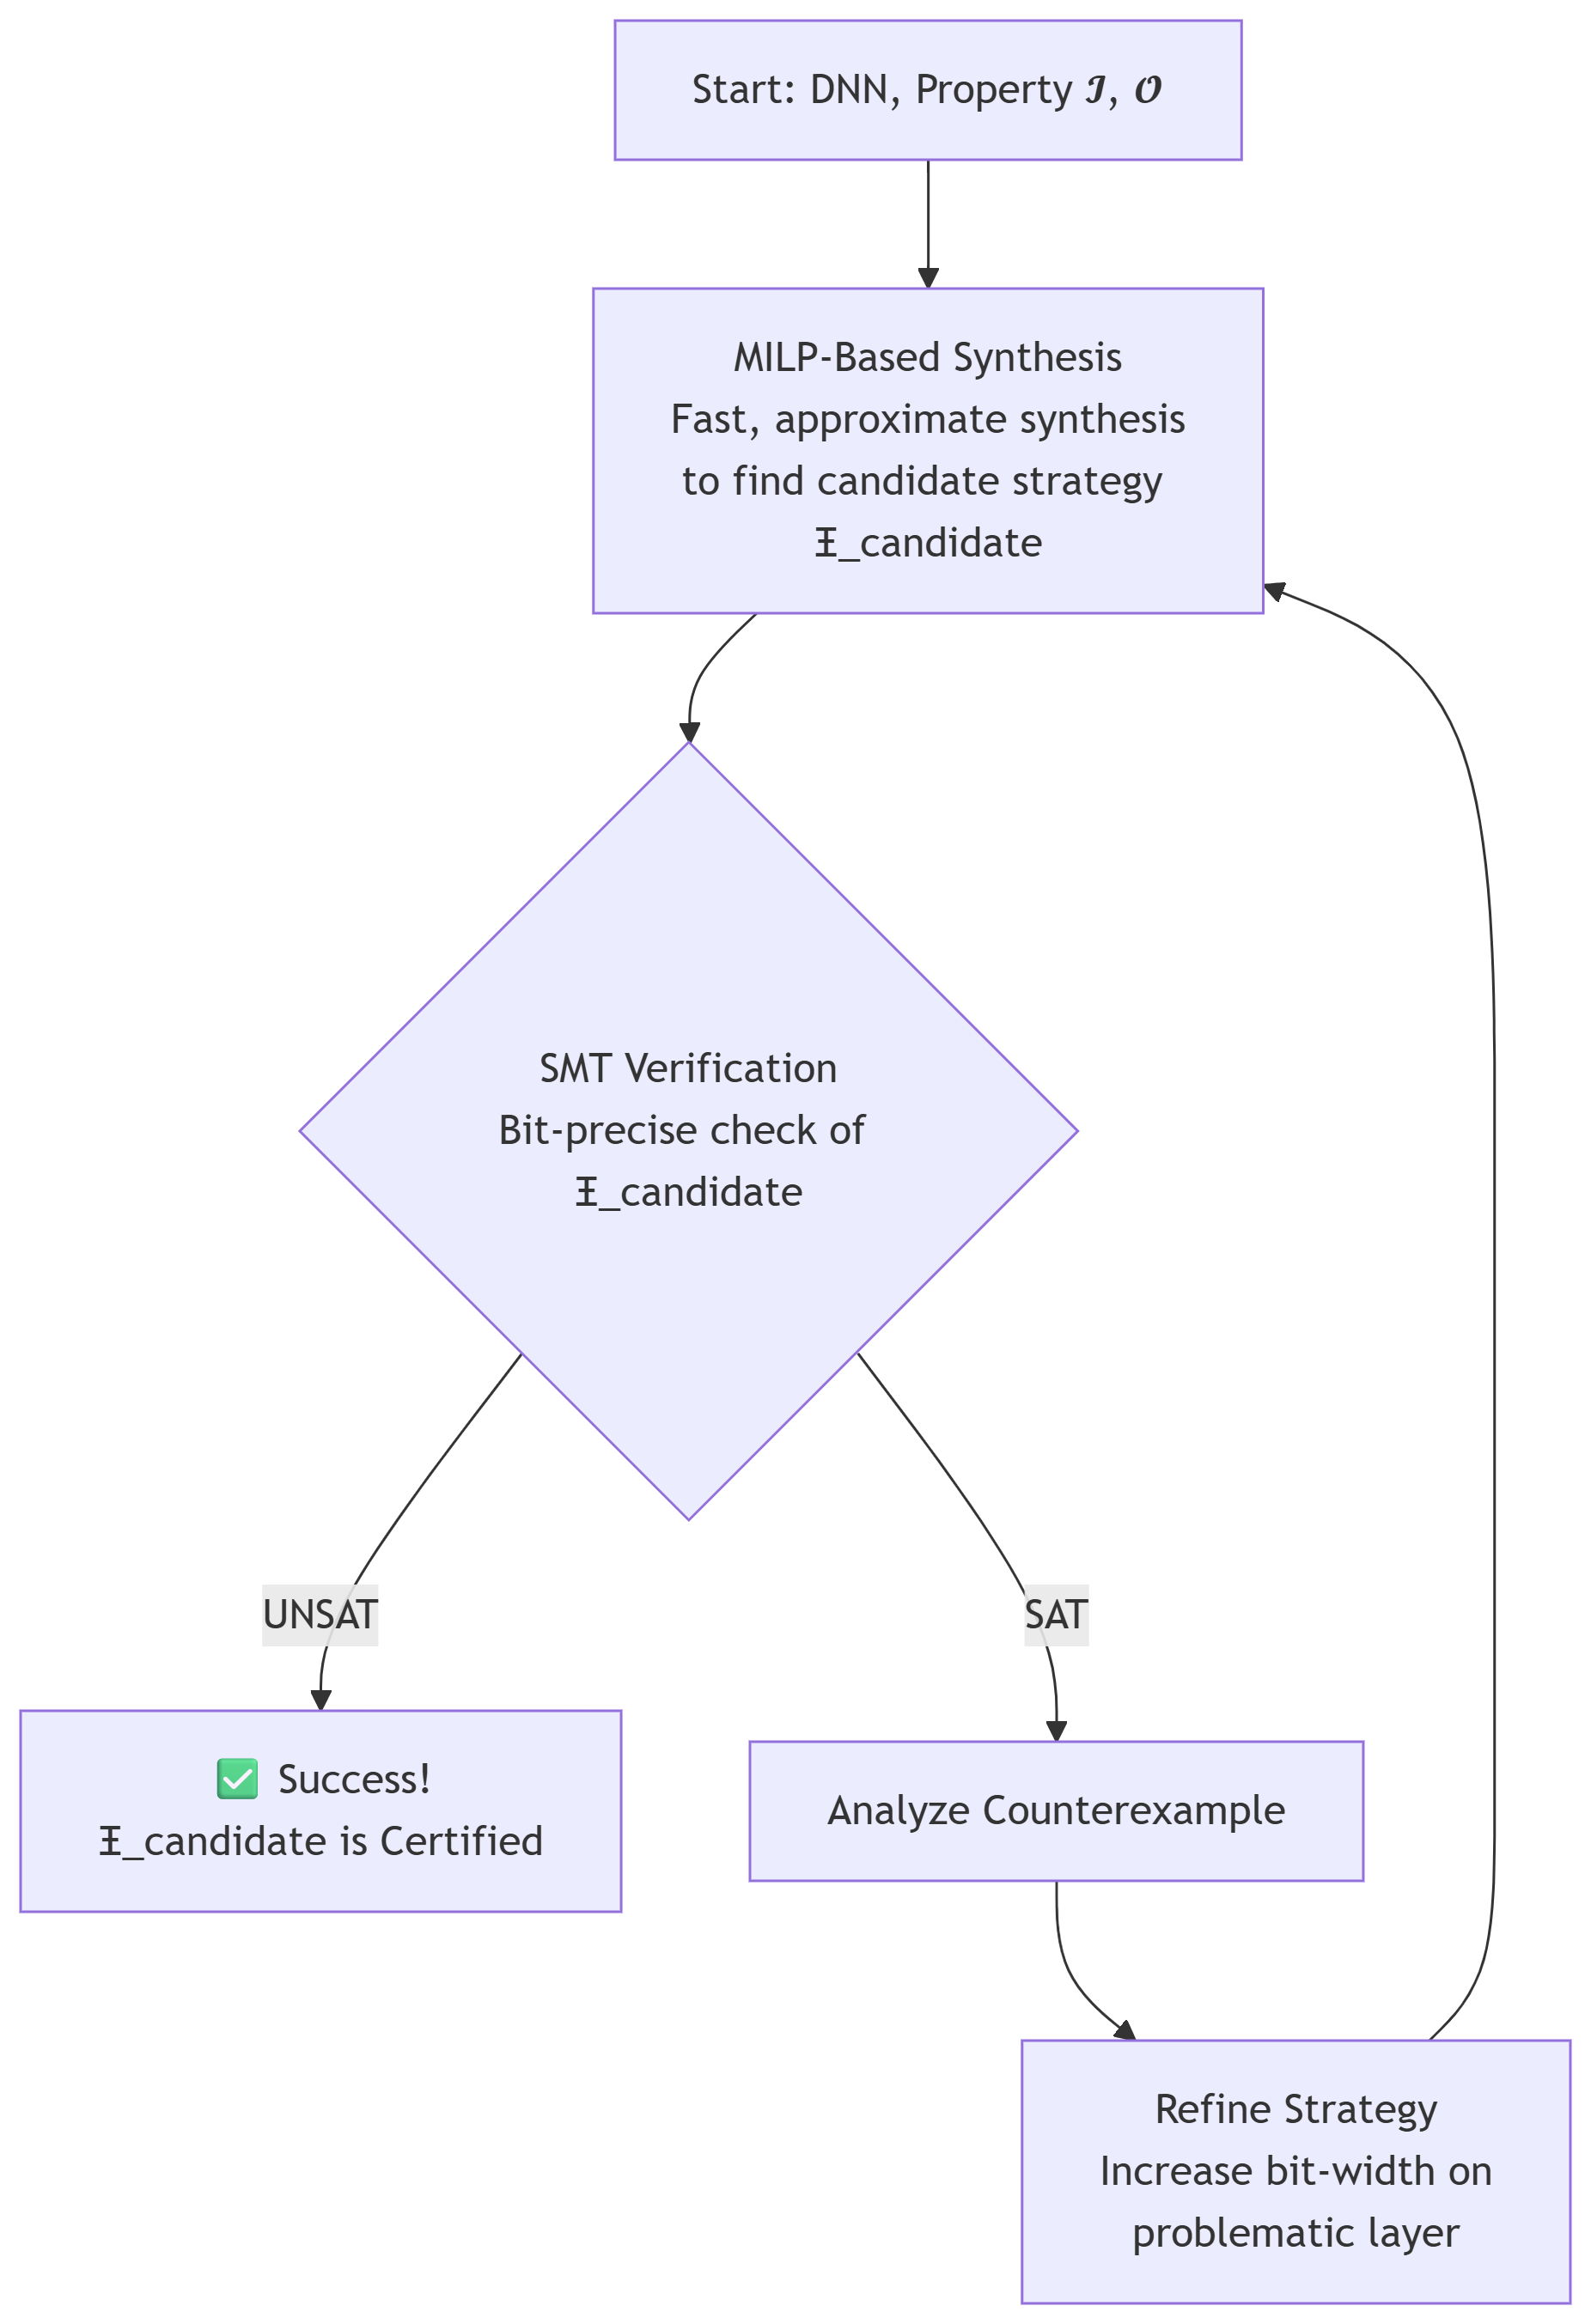
\includegraphics[width=0.3\textwidth]{figuras/3-metodologia/frameworkDiagram.png}
\caption{\textcolor{red}{(POSSIBLE DIAGRAM)}}
\label{fig:frameworkDiagram}
\end{figure}
\newpage
\section{Problem}

ANN are widely used in various applications, but their computational and memory resource demands are high \cite{amir2021smt, han2020understanding, abdi2021counterexample, song2023qnnrepair}. Quantization is a crucial technique to mitigate this problem by reducing the bit-width (from 32-bit floating-point to 8-bit integers or even binary) used to represent weights, biases, and activations, making networks more efficient on embedded and low-power devices \cite{amir2021smt, han2020understanding,song2023qnnrepair, abdi2021counterexample, Cai2020Certified}.

However, quantization introduces an "implementation gap" \cite{cordeiro2025neuralnetworkverificationprogramming}. Most formal verification techniques for neural networks (such as Reluplex and Marabou) assume that networks operate with real-number arithmetic \cite{katz2017reluplex,amir2021smt}. In contrast, actual hardware implementations use finite-precision arithmetic, such as low-precision floating-point or, more frequently, fixed-point \cite{han2020understanding}. This discrepancy means that the safety and correctness guarantees obtained on ideal models may not hold for the deployed neural network \cite{abdi2021counterexample}.

Furthermore, quantization, while beneficial for efficiency, can degrade accuracy and, more critically, compromise desired safety and correctness properties, such as adversarial robustness (resistance to small input perturbations that change the classification) and the absence of backdoors (intentionally inserted vulnerabilities). Existing work on QNN verification generally focuses on post-hoc analyses; that is, they verify a network after it has been quantized \cite{abdi2021counterexample,Cai2020Certified}.

\section{Proposed Approach}

\textcolor{red}{Poderias inserir um diagrama para apresentar a sua metodologia? A partir desse diagrama, você pode descrever cada bloco da metodologia por seções.}

This dissertation proposes the development of a framework for the certified synthesis of quantization strategies that guarantee the preservation of desired properties after quantization, directly addressing finite-precision arithmetic. This differs from post-hoc approaches and quantization techniques that focus solely on accuracy.

\textbf{Synthesis of Quantization Strategies (Inspired by Quadapter):}
The work Quadapter is the first to propose the synthesis of certified quantization strategies \cite{Zhu2021Quadapter,Cai2020Certified}. Its central idea is to compute the pre-image of each layer concerning the desired output region and then identify the minimum bit-width for each layer, ensuring that the quantized layer's reachable region remains within that pre-image.

This dissertation would extend this line of work by focusing on the incorporation of fixed-precision arithmetic during the synthesis process. This is not the primary focus of Quadapter in its current state, which, while dealing with realistic quantization representations, does not yet formally incorporate the nuances of fixed-point arithmetic during verification.

\textbf{Formal Integration of the SMT Theory of Fixed-Point Arithmetic:}
A fundamental contribution would be the use of the SMT Theory of Fixed-Point Arithmetic, as formalized by \cite{baranowski2020smt}. This theory provides a rigorous formalization for fixed-point operations, including rounding modes (roundUp, roundDown) and overflow modes (saturation, wrapAround).

The proposal is to integrate this formal theory into the pre-image calculation and quantization procedures of the synthesis framework. This would allow the synthesized quantization strategies to be certified for the specific finite precision of the hardware, ensuring that properties hold even with the effects of rounding and overflow. The methods of \cite{baranowski2020smt} already include decision procedures for this theory, via both bit-vectors and reals, which is essential for a verifier. They present a case study that utilizes this theory to validate QNNs.

This would more robustly solve the "implementation gap," as the formal guarantees would be directly on the behavior of fixed-point arithmetic, not just a real-number approximation.

\textbf{Pre-image Calculation with Fixed-Point Semantics:}
Quadapter uses a method based on Mixed-Integer Linear Programming (MILP) to compute under-approximations of the pre-image. This dissertation would adapt this MILP formulation to precisely reflect fixed-point operations (including rounding and overflow) instead of just real numbers. This would ensure that the calculated pre-image already accounts for the effects of finite precision.

\textbf{Bit-Precise Verification in Progressive Quantization:}
In Quadapter's progressive quantization algorithm, the verification step $\left(\gamma(\hat{A}_{2i}) \subseteq P_{2i}\right)$ \textcolor{red}{(Still have to add the math theory)} compares the quantized reachable region with the pre-image. The proposal is to use formal SMT-based fixed-point reasoning (potentially through backends like ESBMC) to perform this verification in a bit-precise manner \cite{esbmc2025}. This would mean that the inclusion of the quantized reachable region within the pre-image would be verified considering the exact rules of fixed-point arithmetic.

QNN verification is a PSPACE-hard problem, and scalability is a known challenge for all verifiers (e.g., Marabou, Reluplex, CEG4N). Even Quadapter faces timeouts in pre-image calculations \cite{cai2025certified}.

\textbf{Adaptive/Dynamic Quantization:} While Quadapter synthesizes per-layer bit-widths, this research could explore how to fine-tune precision (e.g., different precisions within a layer, as discussed by \cite{han2020understanding,abdi2021counterexample}) in a verification-guided manner to minimize bit requirements without losing properties, seeking a balance that optimizes verifier performance.

\section{Experimental Methodology}

To empirically validate the certified quantization synthesis methodology proposed in this dissertation, a meticulous selection of public benchmarks, widely recognized in the formal verification of neural networks community, will be used. The choice of benchmarks was designed to ensure a comprehensive evaluation, covering a variety of network architectures, application domains, and safety properties. The basis for this selection includes the challenges proposed by the Neural Network Verification Competition (VNN-COMP) and the test suites made available in foundational works in the field \cite{cordeiro2025neuralnetworkverificationprogramming,abdi2021counterexample}.

The evaluation suite will be composed of the following main components. First, for image classification tasks, we will use models trained on the \textbf{MNIST}, \textbf{CIFAR-10}, and \textbf{Fashion-MNIST} datasets. These range from simple, few-layer networks, ideal for scalability analysis, to complex architectures like LeNet, VGGNet, ResNet-18, and MobileNetV2, allowing the framework to be evaluated in realistic scenarios \cite{han2020understanding, qnsong2023qnnrepairCai2020Certified}. Second, for the domain of safety-critical systems, the \textbf{ACAS Xu} benchmark will be central, given its status as the de facto standard for verifying airborne controllers \cite{katz2017reluplex}. Finally, to enable agile prototyping and debugging, smaller-scale models will be employed, such as those used in the \textbf{fairness} case studies with tabular data and the fixed-point quantized \textbf{Cart-Pole} controller \cite{baranowski2020smt}. The primary focus of the certified synthesis will be the preservation of \textbf{adversarial robustness}, a critical and extensively studied property, with the possibility of extension to other formal specifications.


\section{Expected Contributions}
An innovative framework and methodology for the certified synthesis of bit-precise quantization strategies for neural networks, offering formal guarantees that extend to finite-precision implementations.

A formal and empirical demonstration of the impact of fixed-point arithmetic semantics on the preservation of properties during quantization.

Significant scalability improvements for the verification and synthesis of larger and deeper QNNs by combining the power of SMT with fixed-point theory and optimization techniques.

An extension of the approach to guarantee other critical properties, such as adversarial robustness and the absence of backdoors, beyond the functional equivalence already explored in different contexts (e.g., CEG4N) \cite{abdi2021counterexample}.

This dissertation would fill a critical gap in the research, providing a rigorous foundation for the deployment of safe and reliable neural networks in resource-constrained critical systems.
